\documentclass[a4paper]{article}
\usepackage{caption}
\usepackage{subcaption}
\usepackage{tikz}
\usetikzlibrary{bayesnet}
\usepackage{booktabs}


\setlength{\tabcolsep}{12pt}
\begin{document}
	
	\begin{figure}[ht]
		\begin{center}
			\begin{tabular}{@{}cccc@{}}
				\toprule
				
				$x_N$ explicit & Plate Notation & Hyperparameters on $\mu$ & Factor\\  \midrule
				&                &            &              \\
				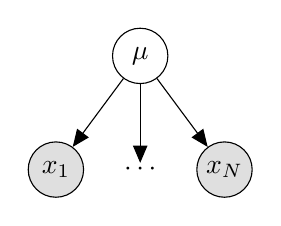
\begin{tikzpicture}
					
					
					\node[obs]                               (x1) {$x_1$};
					\node[const, right=0.5cm of x1]                               (dots) {$\cdots$};
					\node[obs, right=0.5cm of dots]                               (xn) {$x_N$};
					\node[latent, above=of dots] (mu) {$\mathbf{\mu}$};
					
					
					\edge {mu} {x1,dots,xn} ; %
					
				\end{tikzpicture}&
				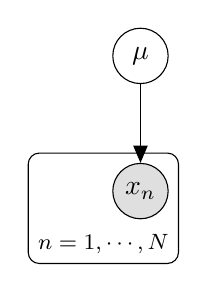
\begin{tikzpicture}
					
					
					\node[obs]                               (xn) {$x_n$};
					\node[latent, above=of xn] (mu) {$\mathbf{\mu}$};
					
					\plate{}{(xn)}{$n = 1, \cdots, N$};
					
					
					\edge {mu} {xn} ; %
					
				\end{tikzpicture} &
				
				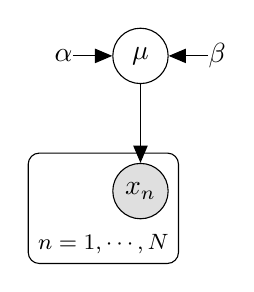
\begin{tikzpicture}
					
					
					\node[obs]                               (xn) {$x_n$};
					\node[latent, above=of xn] (mu) {$\mathbf{\mu}$};
					\node[const, right=0.5cm of mu] (beta) {$\mathbf{\beta}$};
					\node[const, left=0.5cm of mu] (alpha) {$\mathbf{\alpha}$};
					
					\plate{}{(xn)}{$n = 1, \cdots, N$};
					
					
					\edge {mu} {xn} ; %
					\edge {alpha,beta} {mu} ; %
					
					
				\end{tikzpicture}
			& 	
			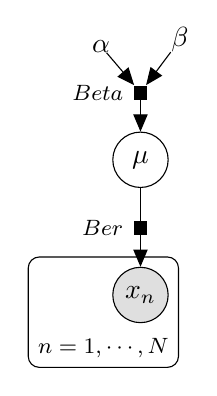
\begin{tikzpicture}
				
				
				\node[obs]                               (xn) {$x_n$};
				\node[latent, above=of xn] (mu) {$\mathbf{\mu}$};
				\factor[above=of xn] {y-f} {left:${Ber}$} {} {} ; %
			\node[const, above=1 of mu, xshift=0.5cm] (beta) {$\mathbf{\beta}$};
				\node[const, above=1 of mu, xshift=-0.5cm] (alpha) {$\mathbf{\alpha}$};
				\factor[above=of mu] {mu-f} {left:${Beta}$} {} {} ; %
				\plate{}{(xn)}{$n = 1, \cdots, N$};
				
				
				
				\edge {mu} {xn} ; %
				\edge {alpha,beta} {mu-f} ; %
				\edge  {mu-f}{mu} ; %
				
				
			\end{tikzpicture}
			
				
			\end{tabular}
			
		\end{center}
		\caption{Graphical models for a repeated Bernoulli experiment.}
	\end{figure}

	
\end{document}